% Research Diary Collection Template for Research Student (University), 2025
\documentclass[letterpaper,11pt]{article}
\newcommand{\userName}{Research Student}
\newcommand{\institution}{University}
\newcommand{\workingDate}{2025 Research Diary}
% Modular package loading - choose what you need
% Files are symlinked in output directory for self-contained compilation

\usepackage{assets/styles/diary_base}        % Core packages and basic theorems
\usepackage{assets/styles/diary_ctheorems}   % Enhanced colored theorem environments
\usepackage{assets/styles/diary_commands}   % Personal shortcuts and commands

\usepackage{tocloft}
\setlength{\cftbeforesecskip}{5pt}
\renewcommand*\contentsname{Research Student's Research Diary -- Contents}

\title{Research Diary Collection - 2025}
\author{Research Student}
\date{Compiled \today}

\begin{document}

\tableofcontents
\thispagestyle{empty}
\newpage


% Entry from 2025-09-20-newmethod.tex
\href{run:2025-09-20-newmethod.tex}{\Huge September 20} 

\section{Citation Test}


We have a citation \cite{research_methods2024} here.  Solve this problem: 



\clearpage


% Entry from 2025-09-20.tex
\href{run:2025-09-20.tex}{\Huge September 20} 

\section{Rectified Flow}

We have a figure here. 
\begin{figure}[h]
\centering 
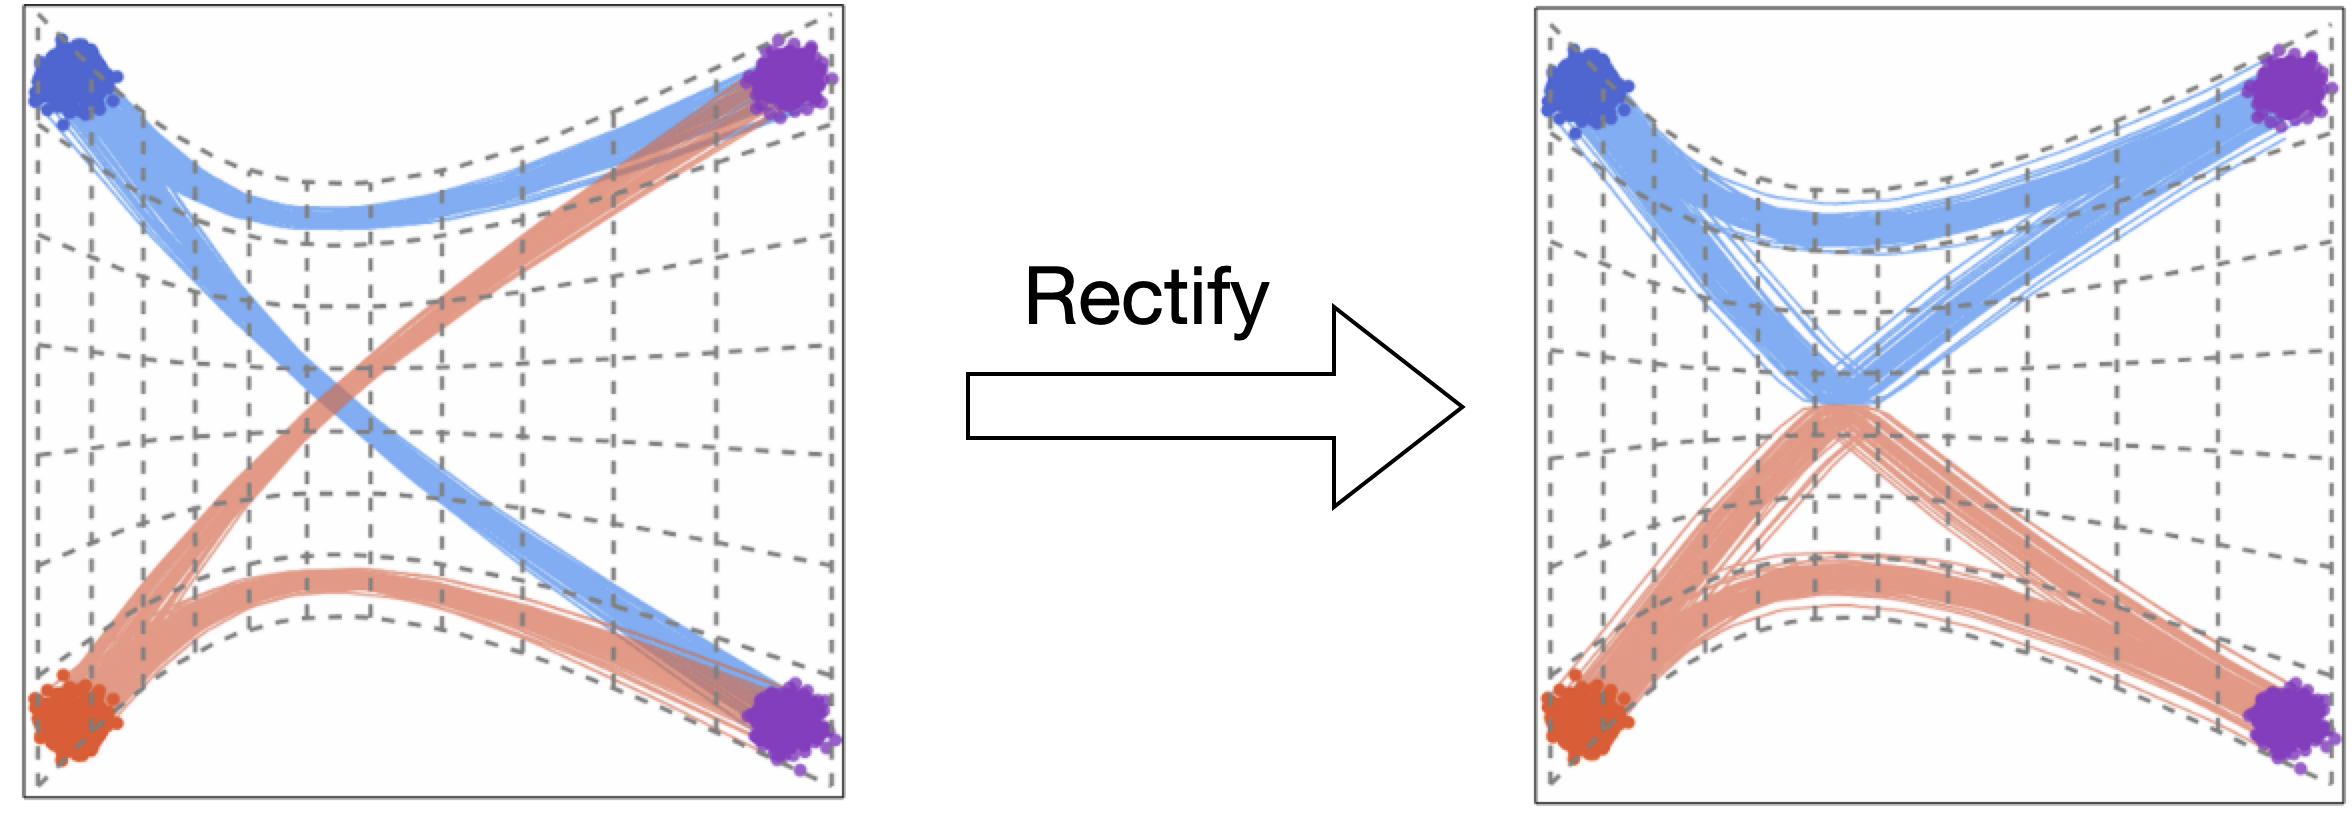
\includegraphics[width=0.8\textwidth]{assets/figures/2025/curved_reflow.png}
\end{figure} 


We have another citation here \cite{li2022diffusion}. 


\clearpage


% Entry from 2025-09-21-momentum_cwd-EXPANDED.tex
\href{run:2025-09-21-momentum_cwd.tex}{\Huge September 21} 

\section{Momentum + Cautious WD}

\begin{align}
    \dot x = - m - \mathbb{I}(mx\geq 0) x \\ 
    \dot m = \nabla f(x) - m. 
\end{align}
$$
H(x, m) = f(x) + \frac{1}{2} m^2 + (mx)_+
$$

Let us use $s \in[0,1]$ to denote the subgradient of $(mx)_+$ within $H$. Let $p \in[0,1]$ be the Flippiov variable of $\mathbb{I}(mx \geq 0)$ inside the velocity field. Note that $s$ and $p$ are different. We need to keep track of it in the derivation. 
\begin{align*}
\dot H(s,p) &  =  g \dot x + m \dot m + s (m \dot x + x \dot m) \\ 
& = -g (m + p x) + m(g - m) + s (-m (m + p x) + x (g - m) )\\
& = - p x g - m^2 + s (- m^2 + xg - (1+p)xm)
\end{align*}

If $\alpha$ belongs to $\dot H$, we want that for each $s$, there exists $p$, such that 
$$
- p x g - m^2 + s (- m^2 + xg - (1+p)xm) = -\alpha.
$$
So we have 
$$
p (-xg - s x m ) - m^2 + s (-m^2 + xg - xm) = \alpha. 
$$
$$
p = \frac{\alpha -(1+s) m^2 + s (xg - xm)}{xg +  s xm}. 
$$
At the non-smooth point, we have $xm =0$, and it gives 
$$
p = \frac{\alpha -(1+s) m^2 + s (xg)}{xg}.  
$$
So $p$ is in range of 
$$
\frac{\alpha - 2m^2 + xg}{xg}, ~~~~ 
\frac{\alpha - m^2 }{xg}. 
$$
If $xg >0$, we have 
$$
m^2 \leq \alpha \leq m^2 + xg
$$
$$
\alpha \leq 2m^2 \leq \alpha + xg 
$$
So 
$$
2m^2  - xg \leq \alpha \leq 2 m^2
$$

$$\cap_{s} \cup_{p} \dot H(s, p).$$


For know the flippov system, the set valued Lie-derivation is defined as:
$$
\mathcal L_v H  =   
\{\alpha \colon \exists p, ~~~ s.t. ~~~ \dot H(s,p) = \alpha ~~~\forall s \in \partial H \}.
$$
So we want to find the $p$ such that the $\dot H(s,p)$ is independent with the choice of $s$. 

So to make it independent on $s$, we want 
$$
-m^2 + xg -(1+p)xm  = 0.
$$
This gives
\begin{align*}
\dot H 
& = -p(m^2 + (1+p) xm)- m^2 \\
& = -(1+p)m^2 - p(1+p) xm. 
\end{align*}

If $xm <0$, we have $p=0$, and hence $\dot H = - m^2$. 
Invariant set is $\{xm < 0, ~~ m=0\}$.

If $xm >0$, we have $p = 1$, and hence, $\dot H = -(2 m^2 + 2 (xm)_+)$. Invariant set is $\{xm=0, ~~ m=0\}.$

If $xm=0$, we have $\dot H = -(1+p) m^2$. Invariant set is $\{xm=0, m = 0\}$. 

Hence, the invariant set is included in 
$$
\{xm \leq 0, ~~ m = 0\}. 
$$

But since $m=0$, we have $xm\leq 0$ anyway. 


\section{General Fillipov From Scratch}

\begin{ctheorem}
Assume we have non-smooth function $V(x)$ with clark generalized gradient, and let $d$ be an update direction. We have 
\end{ctheorem} 
\begin{cproof} 
\begin{align*}
\lim_{\epsilon \to 0^+}\frac{V(x + \epsilon d) - V(x)}{\epsilon} 
= ... 
\end{align*}  
\end{cproof}   

\begin{thm}[Great Theorem]
    Yes, it is. 
\end{thm}
\begin{proof} 
    Yes. 
\end{proof}    

\begin{theorem}[Great Theorem]
    This is the second. 
\end{theorem}
\begin{proof}
    This is the best. 
\end{proof}     





\clearpage


% Entry from 2025-09-21-momentum_cwd-clean.tex
\href{run:2025-09-21-momentum_cwd.tex}{\Huge September 21} 

\section{Momentum + Cautious WD}

\bb
\dot x + \RR^d + \dd f + \E[x]. 
\ee 

\begin{align}
    \dot x = - m - \ind(mx\geq 0) x \\ 
    \dot m = \dd f(x) - m. 
\end{align}
$$
H(x, m) = f(x) + \frac{1}{2} m^2 + (mx)_+
$$

Let us use $s \in[0,1]$ to denote the subgradient of $(mx)_+$ within $H$. Let $p \in[0,1]$ be the Flippiov variable of $\ind(mx \geq 0)$ inside the velocity field. Note that $s$ and $p$ are different. We need to keep track of it in the derivation. 
\begin{align*}
\dot H(s,p) &  =  g \dot x + m \dot m + s (m \dot x + x \dot m) \\ 
& = -g (m + p x) + m(g - m) + s (-m (m + p x) + x (g - m) )\\
& = - p x g - m^2 + s (- m^2 + xg - (1+p)xm)
%(g + sm) \dot x + (m + s x) \dot m 
\end{align*}

%We want 
If $\alpha$ belongs to $\dot H$, we want that for each $s$, there exists $p$, such that 
$$
- p x g - m^2 + s (- m^2 + xg - (1+p)xm) = -\alpha.
$$
So we have 
$$
p (-xg - s x m ) - m^2 + s (-m^2 + xg - xm) = \alpha. 
$$
$$
p = \frac{\alpha -(1+s) m^2 + s (xg - xm)}{xg +  s xm}. 
$$
At the non-smooth point, we have $xm =0$, and it gives 
$$
p = \frac{\alpha -(1+s) m^2 + s (xg)}{xg}.  
$$
So $p$ is in range of 
$$
\frac{\alpha - 2m^2 + xg}{xg}, ~~~~ 
\frac{\alpha - m^2 }{xg}. 
$$
If $xg >0$, we have 
$$
m^2 \leq \alpha \leq m^2 + xg
$$
$$
\alpha \leq 2m^2 \leq \alpha + xg 
$$
So 
$$
2m^2  - xg \leq \alpha \leq 2 m^2
$$

$$\cap_{s} \cup_{p} \dot H(s, p).$$


For know the flippov system, the set valued Lie-derivation is defined as:
$$
\mathcal L_v H  =   
\{\alpha \colon \exists p, ~~~ s.t. ~~~ \dot H(s,p) = \alpha ~~~\forall s \in \partial H \}.
$$
So we want to find the $p$ such that the $\dot H(s,p)$ is independent with the choice of $s$. 

So to make it independent on $s$, we want 
$$
-m^2 + xg -(1+p)xm  = 0.
$$
This gives
\begin{align*}
\dot H 
& = -p(m^2 + (1+p) xm)- m^2 \\
& = -(1+p)m^2 - p(1+p) xm. 
\end{align*}

If $xm <0$, we have $p=0$, and hence $\dot H = - m^2$. 
Invariant set is $\{xm < 0, ~~ m=0\}$.

If $xm >0$, we have $p = 1$, and hence, $\dot H = -(2 m^2 + 2 (xm)_+)$. Invariant set is $\{xm=0, ~~ m=0\}.$

If $xm=0$, we have $\dot H = -(1+p) m^2$. Invariant set is $\{xm=0, m = 0\}$. 

Hence, the invariant set is included in 
$$
\{xm \leq 0, ~~ m = 0\}. 
$$

But since $m=0$, we have $xm\leq 0$ anyway. 


\section{General Fillipov From Scratch}

\begin{ctheorem}
Assume we have non-smooth function $V(x)$ with clark generalized gradient, and let $d$ be an update direction. We have 
\end{ctheorem} 
\begin{cproof} 
\begin{align*}
\lim_{\epsilon \to 0^+}\frac{V(x + \epsilon d) - V(x)}{\epsilon} 
= ... 
\end{align*}  
\end{cproof}   

\begin{thm}[Great Theorem]
    Yes, it is. 
\end{thm}
\begin{proof} 
    Yes. 
\end{proof}    

\begin{theorem}[Great Theorem]
    This is the second. 
\end{theorem}
\begin{proof}
    This is the best. 
\end{proof}     





\clearpage


% Entry from 2025-09-21-momentum_cwd.tex
\href{run:2025-09-21-momentum_cwd.tex}{\Huge September 21} 

\section{Momentum + Cautious WD}

\begin{align}
    \dot x = - m - \ind(mx\geq 0) x \\ 
    \dot m = \dd f(x) - m. 
\end{align}
$$
H(x, m) = f(x) + \frac{1}{2} m^2 + (mx)_+
$$

Let us use $s \in[0,1]$ to denote the subgradient of $(mx)_+$ within $H$. Let $p \in[0,1]$ be the Flippiov variable of $\ind(mx \geq 0)$ inside the velocity field. Note that $s$ and $p$ are different. We need to keep track of it in the derivation. 
\begin{align*}
\dot H(s,p) &  =  g \dot x + m \dot m + s (m \dot x + x \dot m) \\ 
& = -g (m + p x) + m(g - m) + s (-m (m + p x) + x (g - m) )\\
& = - p x g - m^2 + s (- m^2 + xg - (1+p)xm)
%(g + sm) \dot x + (m + s x) \dot m 
\end{align*}

%We want 
If $\alpha$ belongs to $\dot H$, we want that for each $s$, there exists $p$, such that 
$$
- p x g - m^2 + s (- m^2 + xg - (1+p)xm) = -\alpha.
$$
So we have 
$$
p (-xg - s x m ) - m^2 + s (-m^2 + xg - xm) = \alpha. 
$$
$$
p = \frac{\alpha -(1+s) m^2 + s (xg - xm)}{xg +  s xm}. 
$$
At the non-smooth point, we have $xm =0$, and it gives 
$$
p = \frac{\alpha -(1+s) m^2 + s (xg)}{xg}.  
$$
So $p$ is in range of 
$$
\frac{\alpha - 2m^2 + xg}{xg}, ~~~~ 
\frac{\alpha - m^2 }{xg}. 
$$
If $xg >0$, we have 
$$
m^2 \leq \alpha \leq m^2 + xg
$$
$$
\alpha \leq 2m^2 \leq \alpha + xg 
$$
So 
$$
2m^2  - xg \leq \alpha \leq 2 m^2
$$

$$\cap_{s} \cup_{p} \dot H(s, p).$$


For know the flippov system, the set valued Lie-derivation is defined as:
$$
\mathcal L_v H  =   
\{\alpha \colon \exists p, ~~~ s.t. ~~~ \dot H(s,p) = \alpha ~~~\forall s \in \partial H \}.
$$
So we want to find the $p$ such that the $\dot H(s,p)$ is independent with the choice of $s$. 

So to make it independent on $s$, we want 
$$
-m^2 + xg -(1+p)xm  = 0.
$$
This gives
\begin{align*}
\dot H 
& = -p(m^2 + (1+p) xm)- m^2 \\
& = -(1+p)m^2 - p(1+p) xm. 
\end{align*}

If $xm <0$, we have $p=0$, and hence $\dot H = - m^2$. 
Invariant set is $\{xm < 0, ~~ m=0\}$.

If $xm >0$, we have $p = 1$, and hence, $\dot H = -(2 m^2 + 2 (xm)_+)$. Invariant set is $\{xm=0, ~~ m=0\}.$

If $xm=0$, we have $\dot H = -(1+p) m^2$. Invariant set is $\{xm=0, m = 0\}$. 

Hence, the invariant set is included in 
$$
\{xm \leq 0, ~~ m = 0\}. 
$$

But since $m=0$, we have $xm\leq 0$ anyway. 


\section{General Fillipov From Scratch}

\begin{ctheorem}
Assume we have non-smooth function $V(x)$ with clark generalized gradient, and let $d$ be an update direction. We have 
\end{ctheorem} 
\begin{cproof} 
\begin{align*}
\lim_{\epsilon \to 0^+}\frac{V(x + \epsilon d) - V(x)}{\epsilon} 
= ... 
\end{align*}  
\end{cproof}   

\begin{thm}[Great Theorem]
    Yes, it is. 
\end{thm}
\begin{proof} 
    Yes. 
\end{proof}    

\begin{theorem}[Great Theorem]
    This is the second. 
\end{theorem}
\begin{proof}
    This is the best. 
\end{proof}     





\clearpage


% Entry from 2025-09-21.tex
\href{run:2025-09-21.tex}{\Huge September 21} 

\section{Today is a New Day}

Dealing with math, code, people, self. 



\clearpage


\bibliographystyle{apalike}
\bibliography{assets/bib/reference,assets/bib/reference2}


\end{document}
